%\begin{frame}{titel}
%    \pause
%    \begin{columns}
%        \begin{column}{0.5\textwidth}
%            \begin{itemize}
%                \item <->
%                \item <->
%                \item <->
%                \item <->
%                \item <->
%                \item <->
%            \end{itemize}
%        \end{column}
%        \begin{column}{0.5\textwidth}
%            \centering
%            \only <->{
%                \includegraphics[scale=0.25]{images/}\\[-0.5\baselineskip]
%                \hspace{1.5cm}}%\href{www. ...}{[name, paper]}
%             }
%        \end{column}
%    \end{columns}
%\end{frame}
\section{Auswertung der Messdaten und Diskussion}
%\subsection{Photolumineszenz und Direktionalität bei konstanter Temperatur}

\begin{frame}{Photolumineszenz bei \SI{4}{\kelvin}}
    \pause
    \begin{columns}
        \begin{column}{0.5\textwidth}
            \begin{itemize}
                \item <1-> Messung der Photolumineszenz bei $\SI{4}{\kelvin}$ 
                \centering
                \only <2-> {
                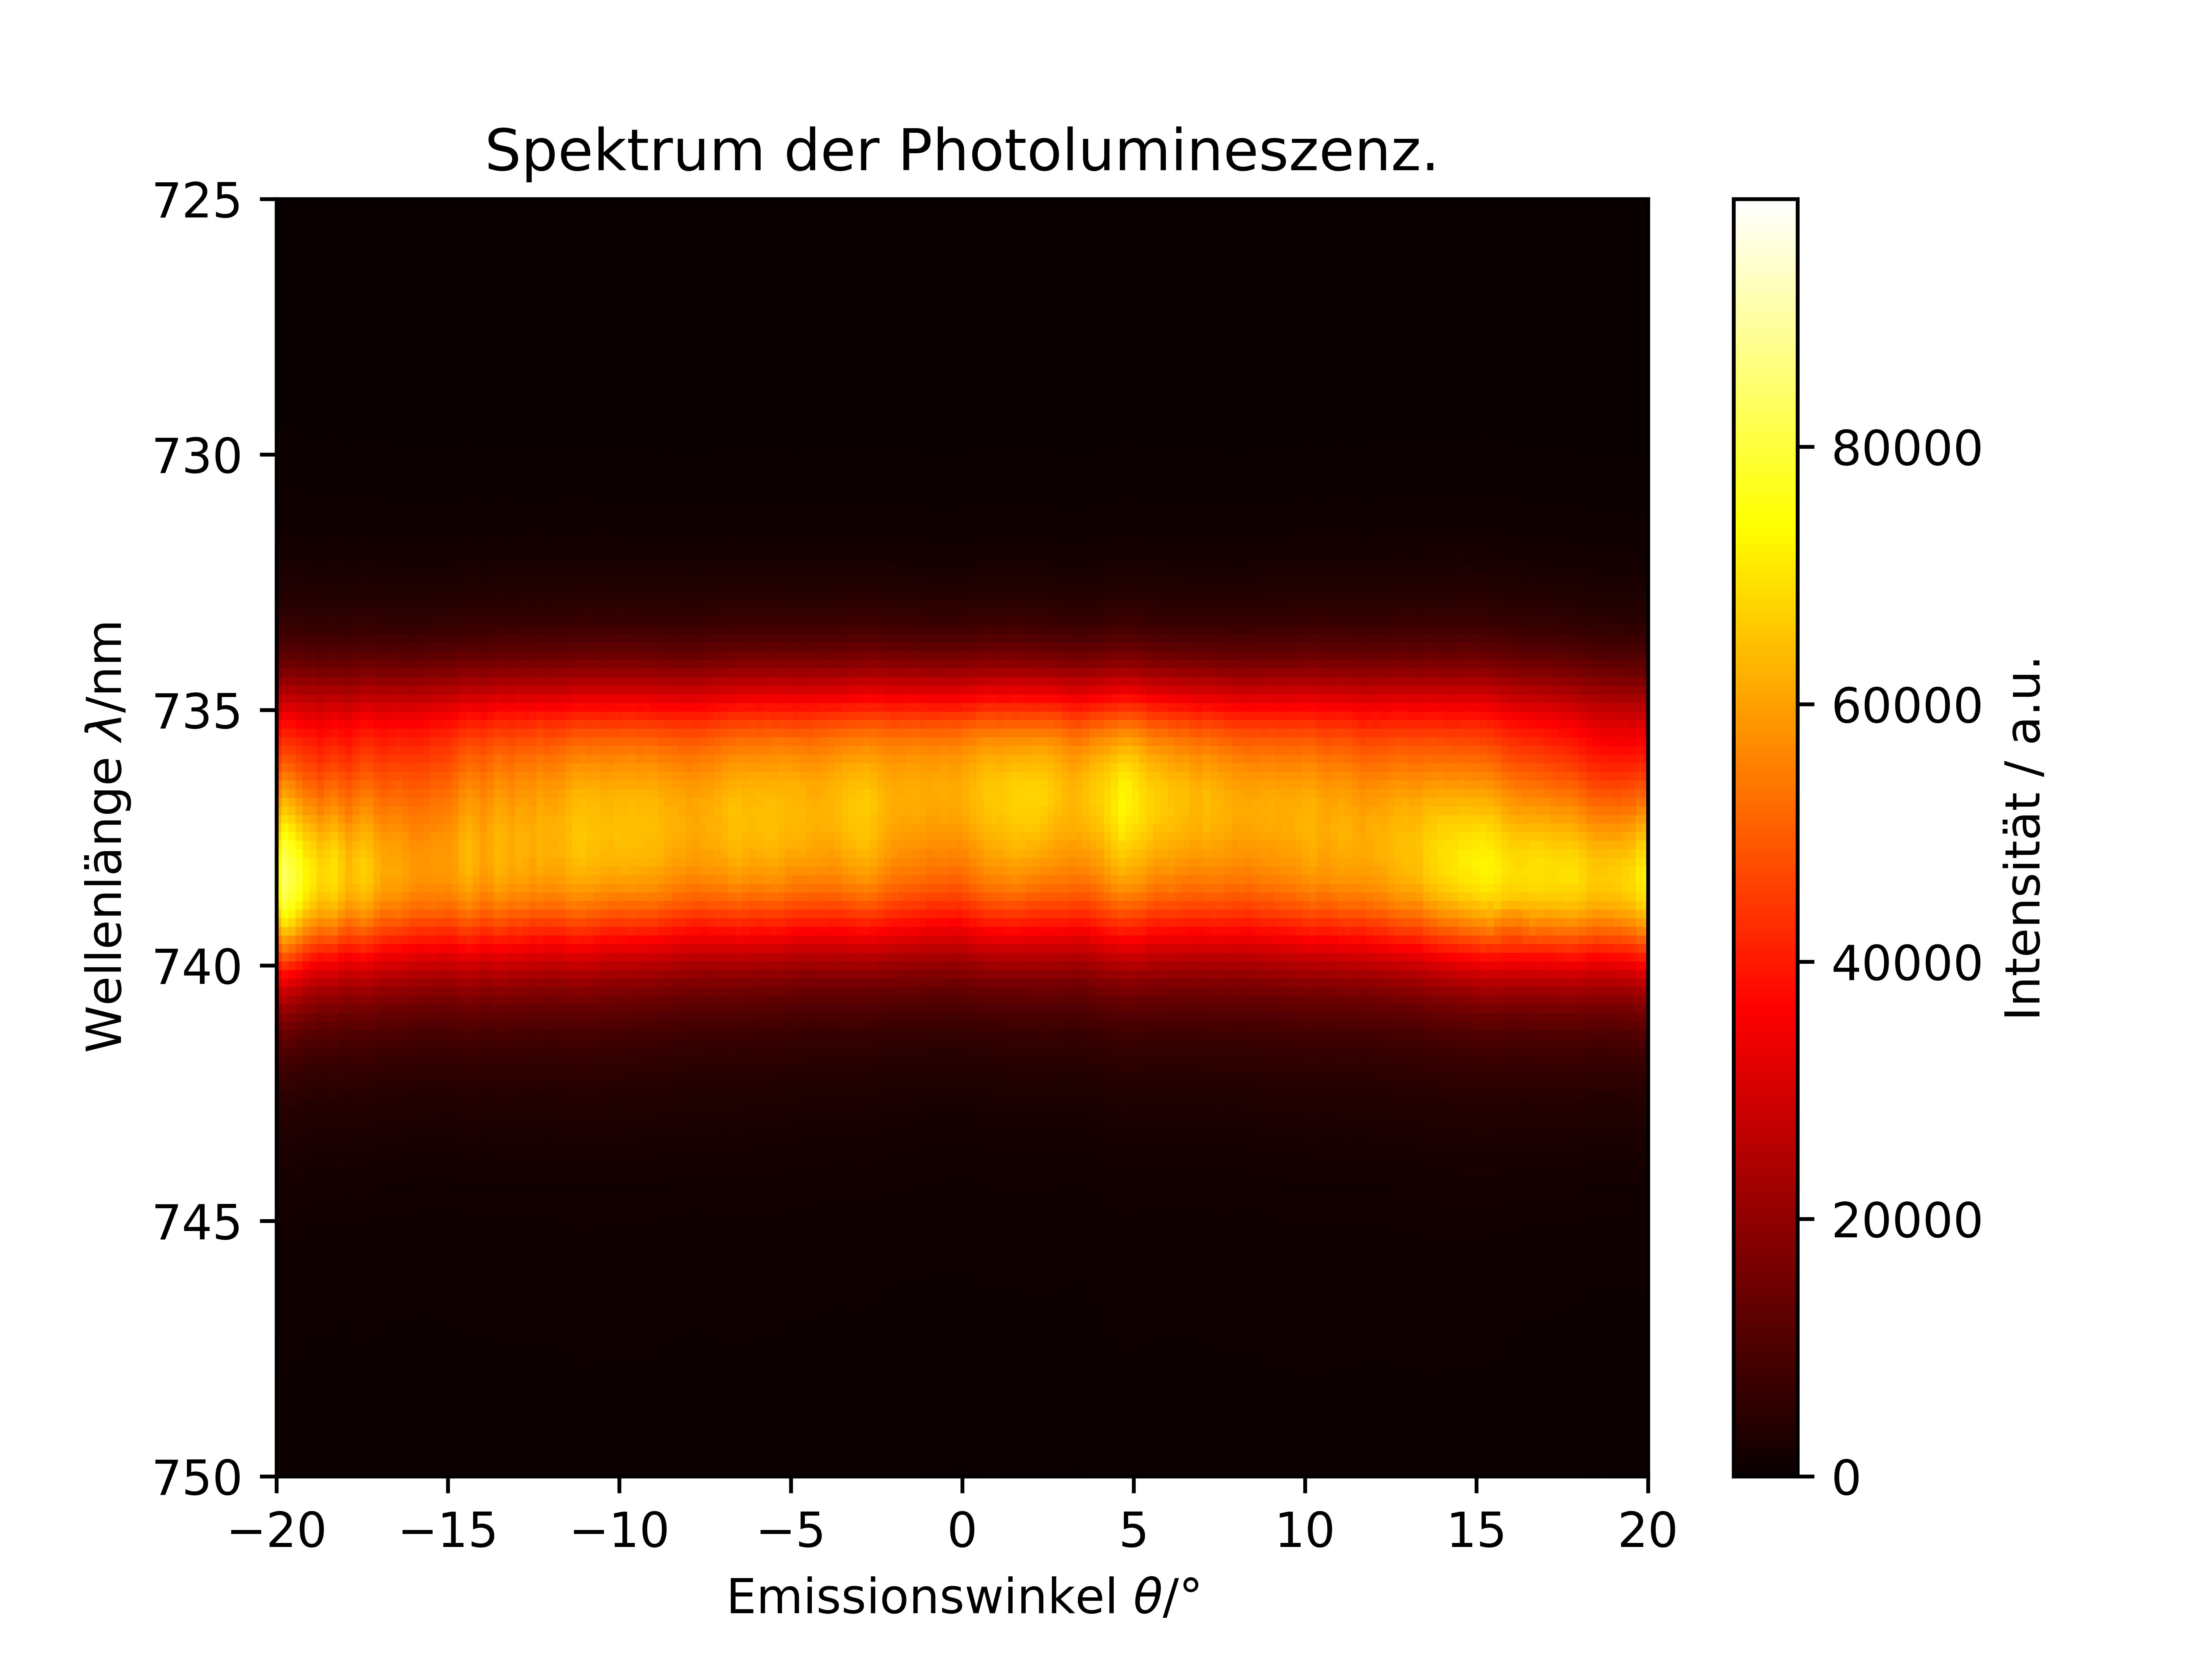
\includegraphics[scale=0.4]{images/colormap__intensity_photolumineszenz_022818A 250nm 4K 2020-07-14.png}\\[-0.5\baselineskip]                
                }
            \end{itemize}
        \end{column}
        \begin{column}{0.5\textwidth}
            \begin{itemize}
                \item <3-> Maximum der Emission bei $\SI{737}{\nano\meter}$ 
                \centering
                \only <3-> {
                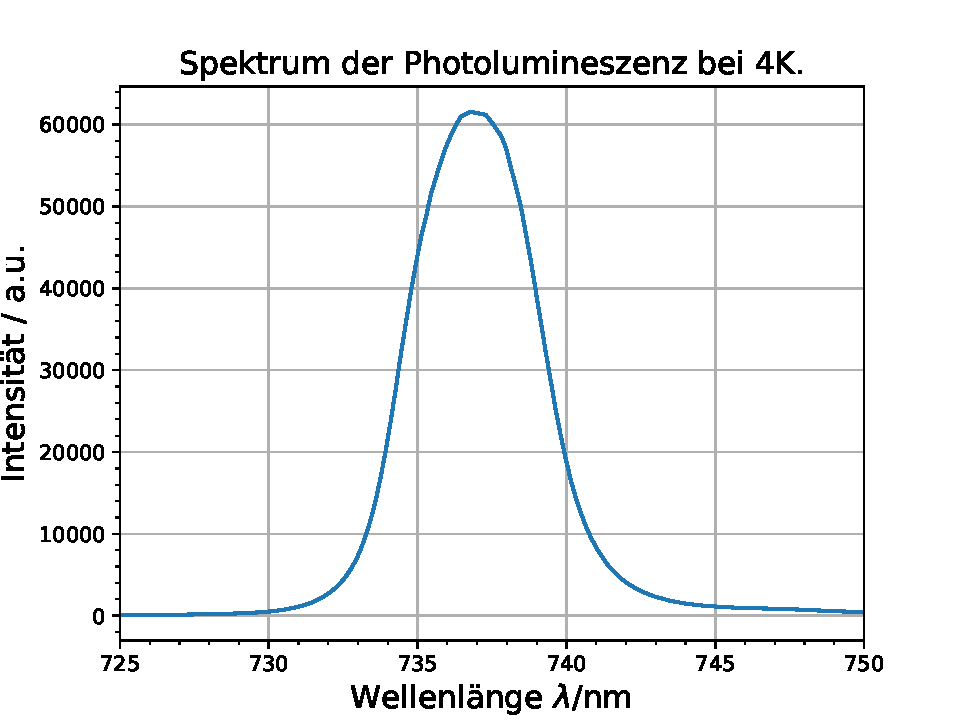
\includegraphics[scale=0.4]{images/max_value_Pl_single.pdf}\\[-0.5\baselineskip]       
                }
            \end{itemize}
        \end{column}
    \end{columns}
\end{frame}

%\begin{frame}{Relative Änderung bei \SI{4}{\kelvin}}
%    \begin{itemize}
%        \item <1-> Richtungsabhängigkeit der Lichtemission
%        \centering
%        \only <1-> {
%        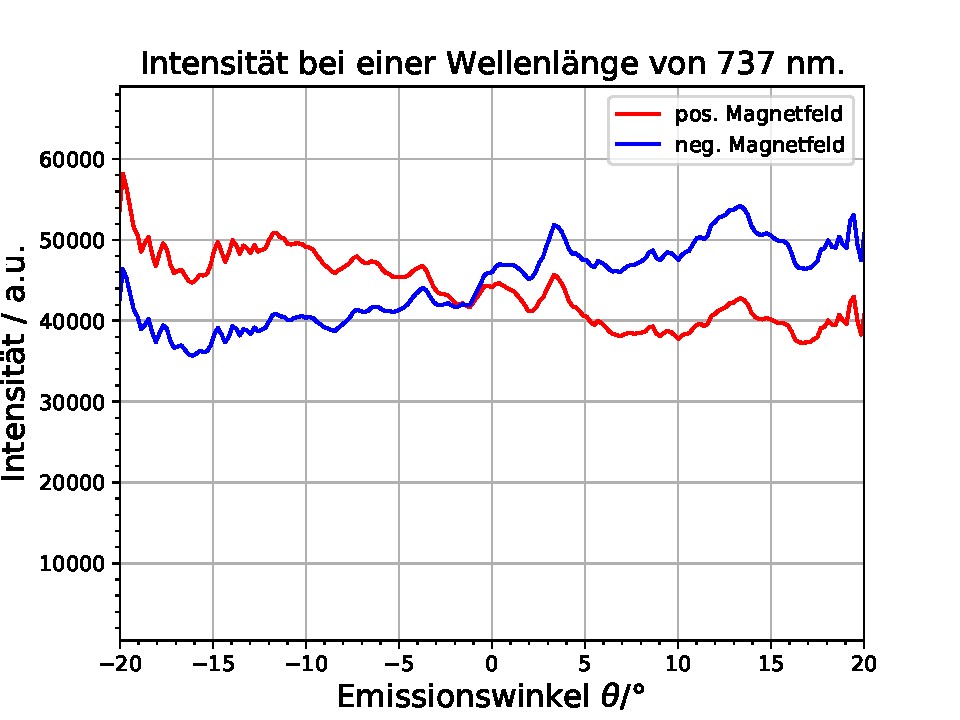
\includegraphics[scale=0.4]{images/positive_and_negative_intensity_at_specific_wavelength_737_nm_022818A 250nm 4K 2020-07-14.pdf}\\[-0.5\baselineskip]                
%        }
%    \end{itemize}
%\end{frame}

\begin{frame}{Relative Änderung bei \SI{4}{\kelvin}}
    \begin{columns}
        \pause
        \begin{column}{0.5\textwidth}
            \begin{itemize}
                \item <2-> Richtungsabhängigkeit der Lichtemission
                \item <3-> Quantifizierung der relativen Änderung der Intensität
                \begin{equation*}
                    \rho = \frac{I_\text{B+} - I_\text{B-} }{ I_\text{B+} + I_\text{B-} }.
                \end{equation*}
                $\rho$ gibt die Änderung der Intensität bei Umpolung des Magnetfelds an.
                \item <6-> Bspl. positive Emissionswinkel \rightarrow relative Änderung $\rho$ negativ 
                \rightarrow mehr Licht bei negativem Magnetfeld emittiert als bei positivem Magnetfeld
                \item <7-> beste Steuerung im Bereich von $\SI{738}{\nano\meter}$ bis $\SI{740}{\nano\meter}$\\
                und $\theta = \pm \SI{11}{\degree}$ bis $\theta = \pm \SI{13,5}{\degree}$
            \end{itemize}
        \end{column}
        \begin{column}{0.5\textwidth}
            \centering 
            \only <1-3> {%
            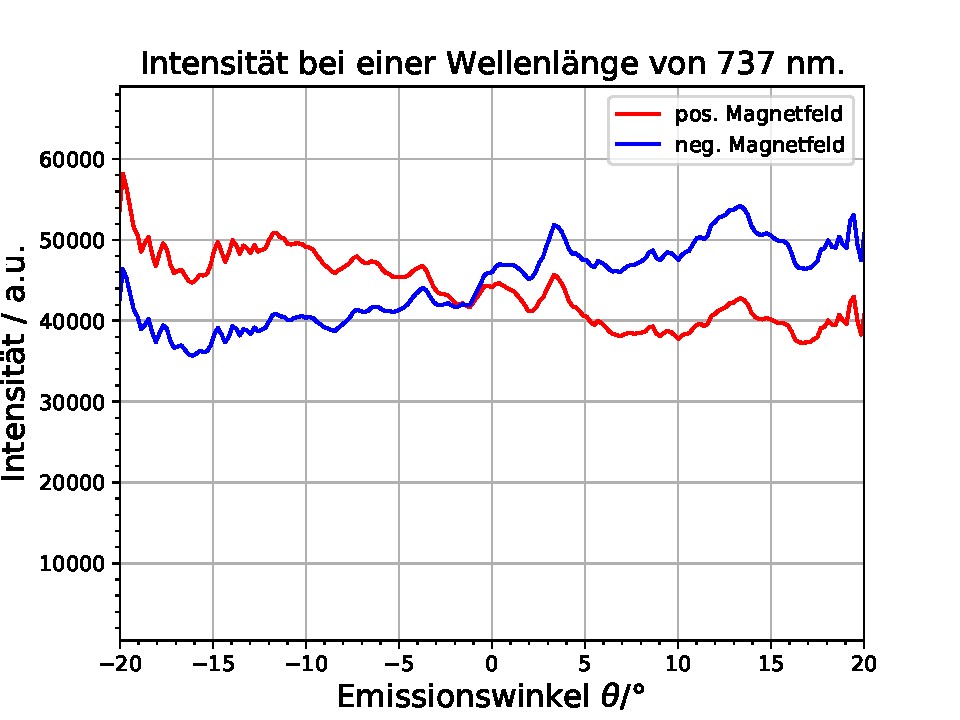
\includegraphics[scale=0.4]{images/positive_and_negative_intensity_at_specific_wavelength_737_nm_022818A 250nm 4K 2020-07-14.pdf}\\[-0.5\baselineskip]%
            }%
            \only <4> {%
            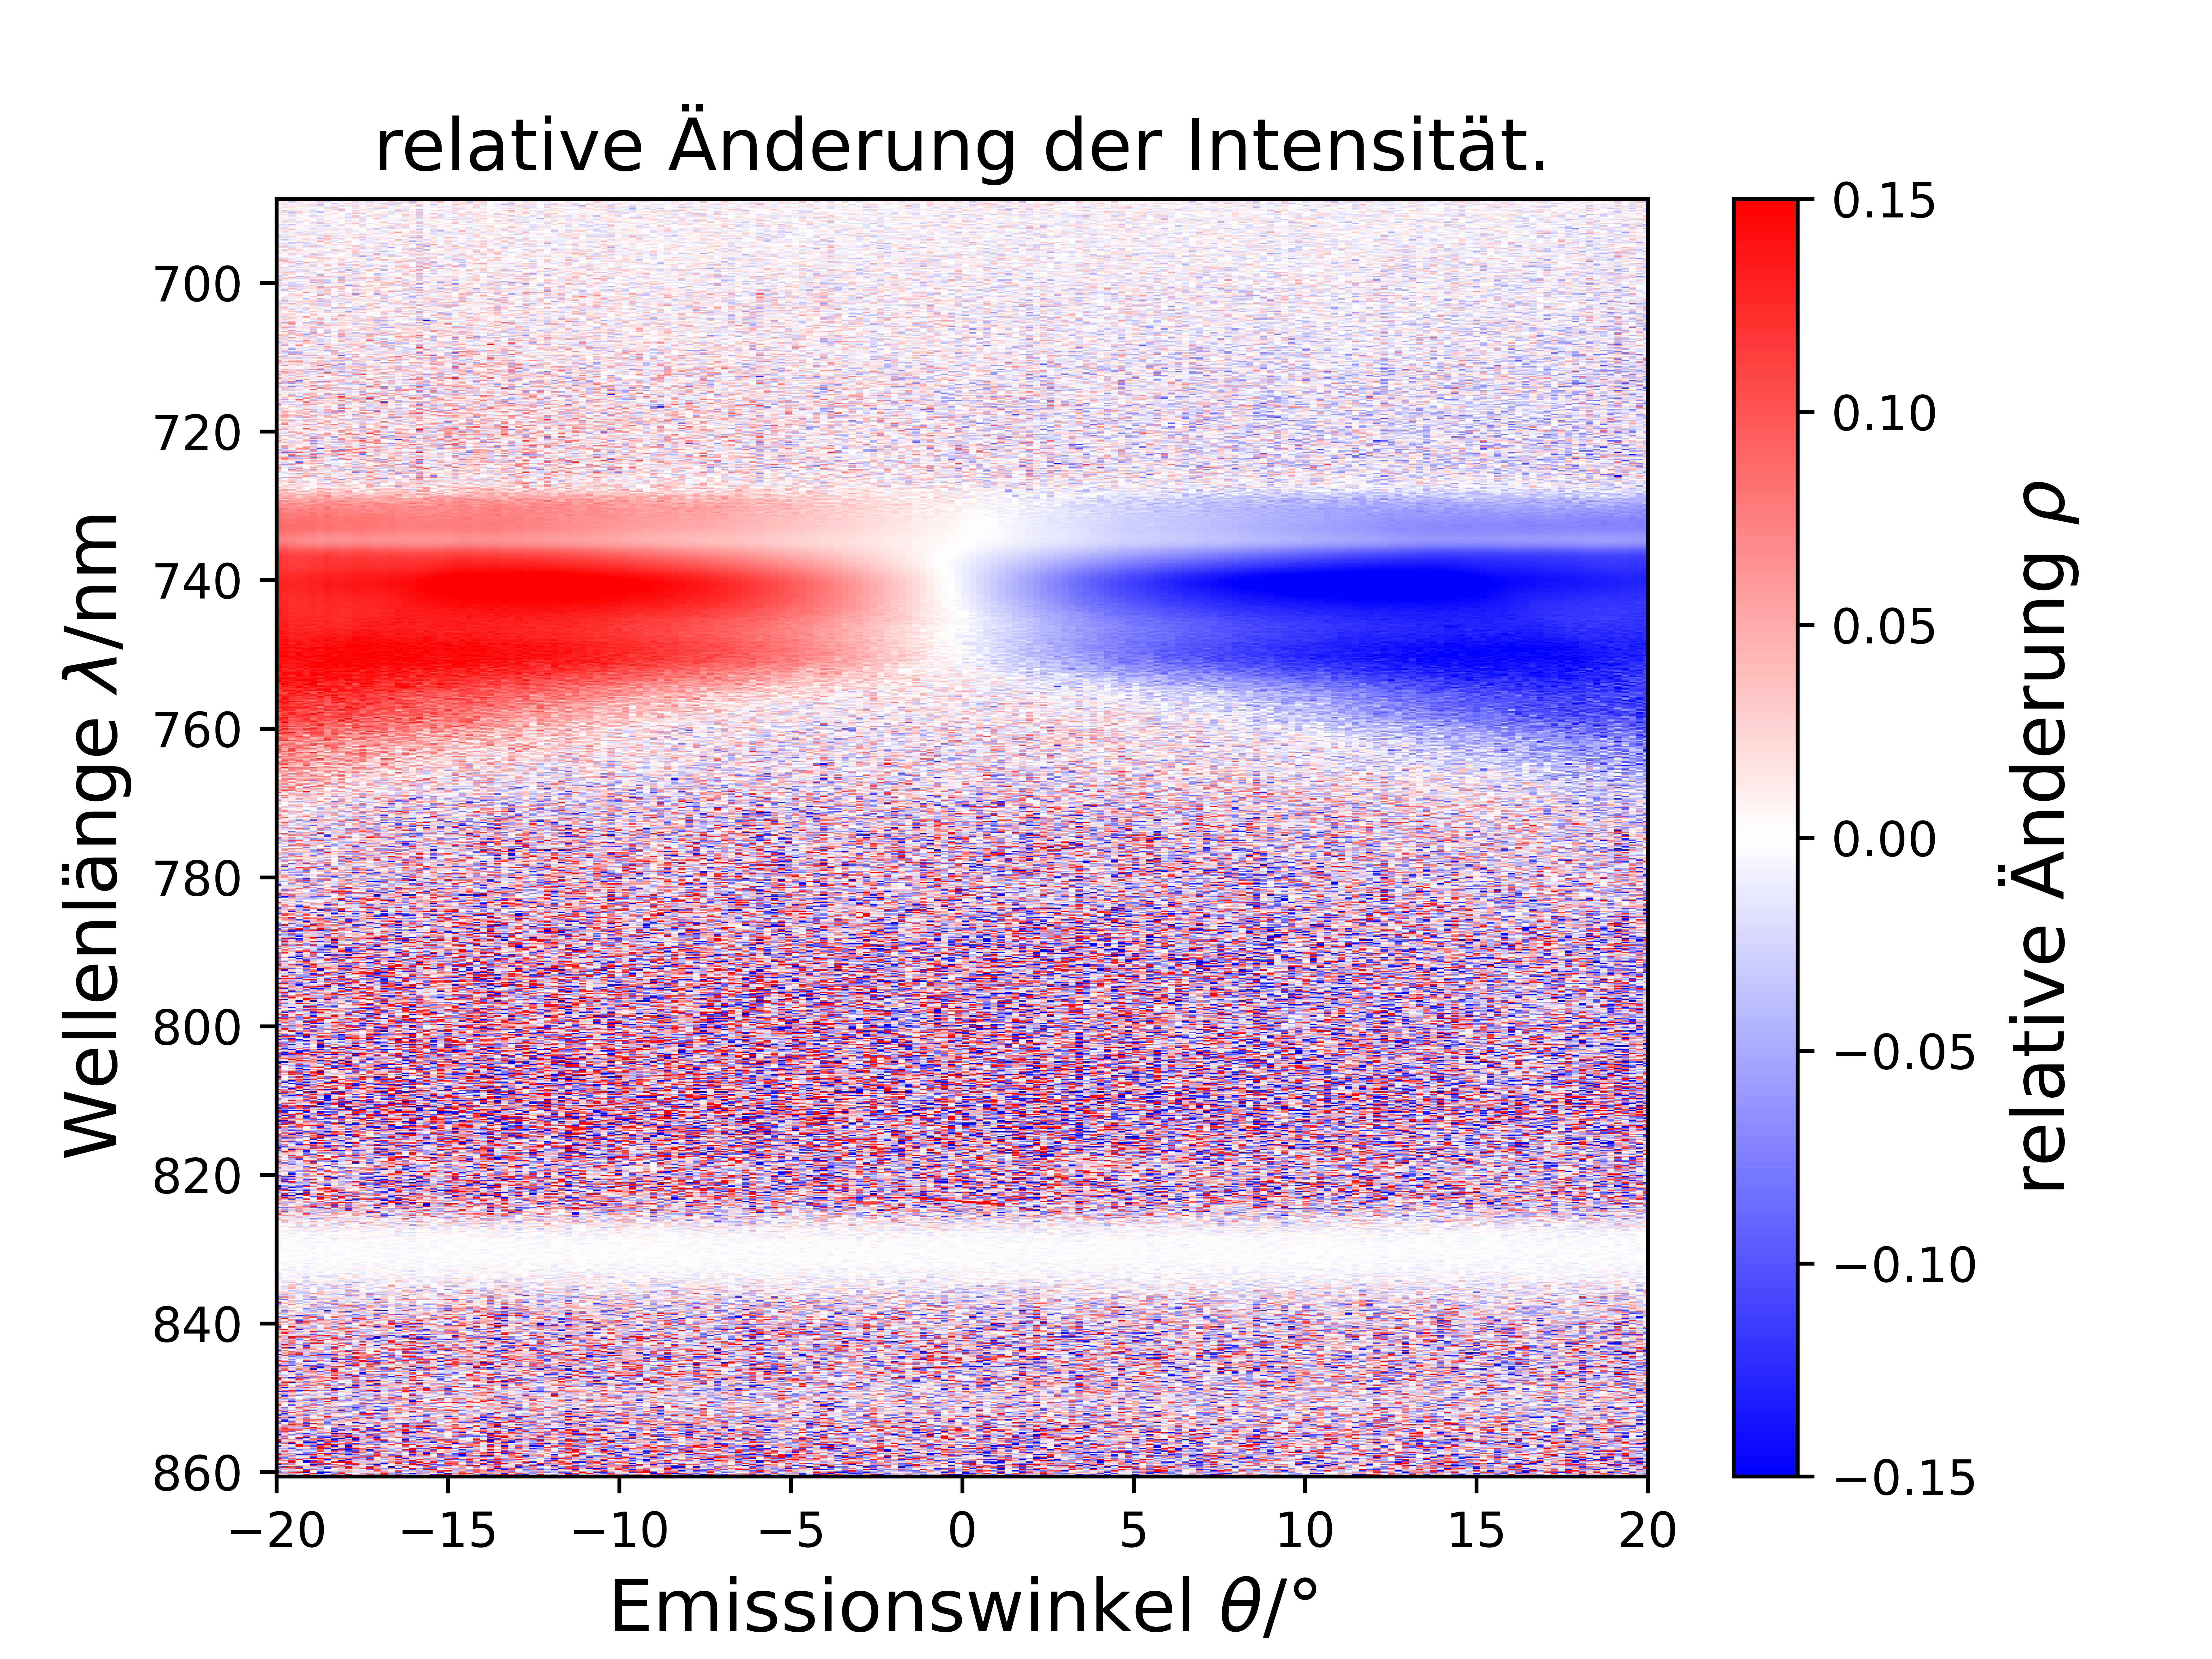
\includegraphics[scale=0.4]{images/colormap_rel_change_intensity_022818A 250nm 4K 2020-07-14_komplett.png}\\[-0.5\baselineskip]%
            }%
            \only <5-> {%
            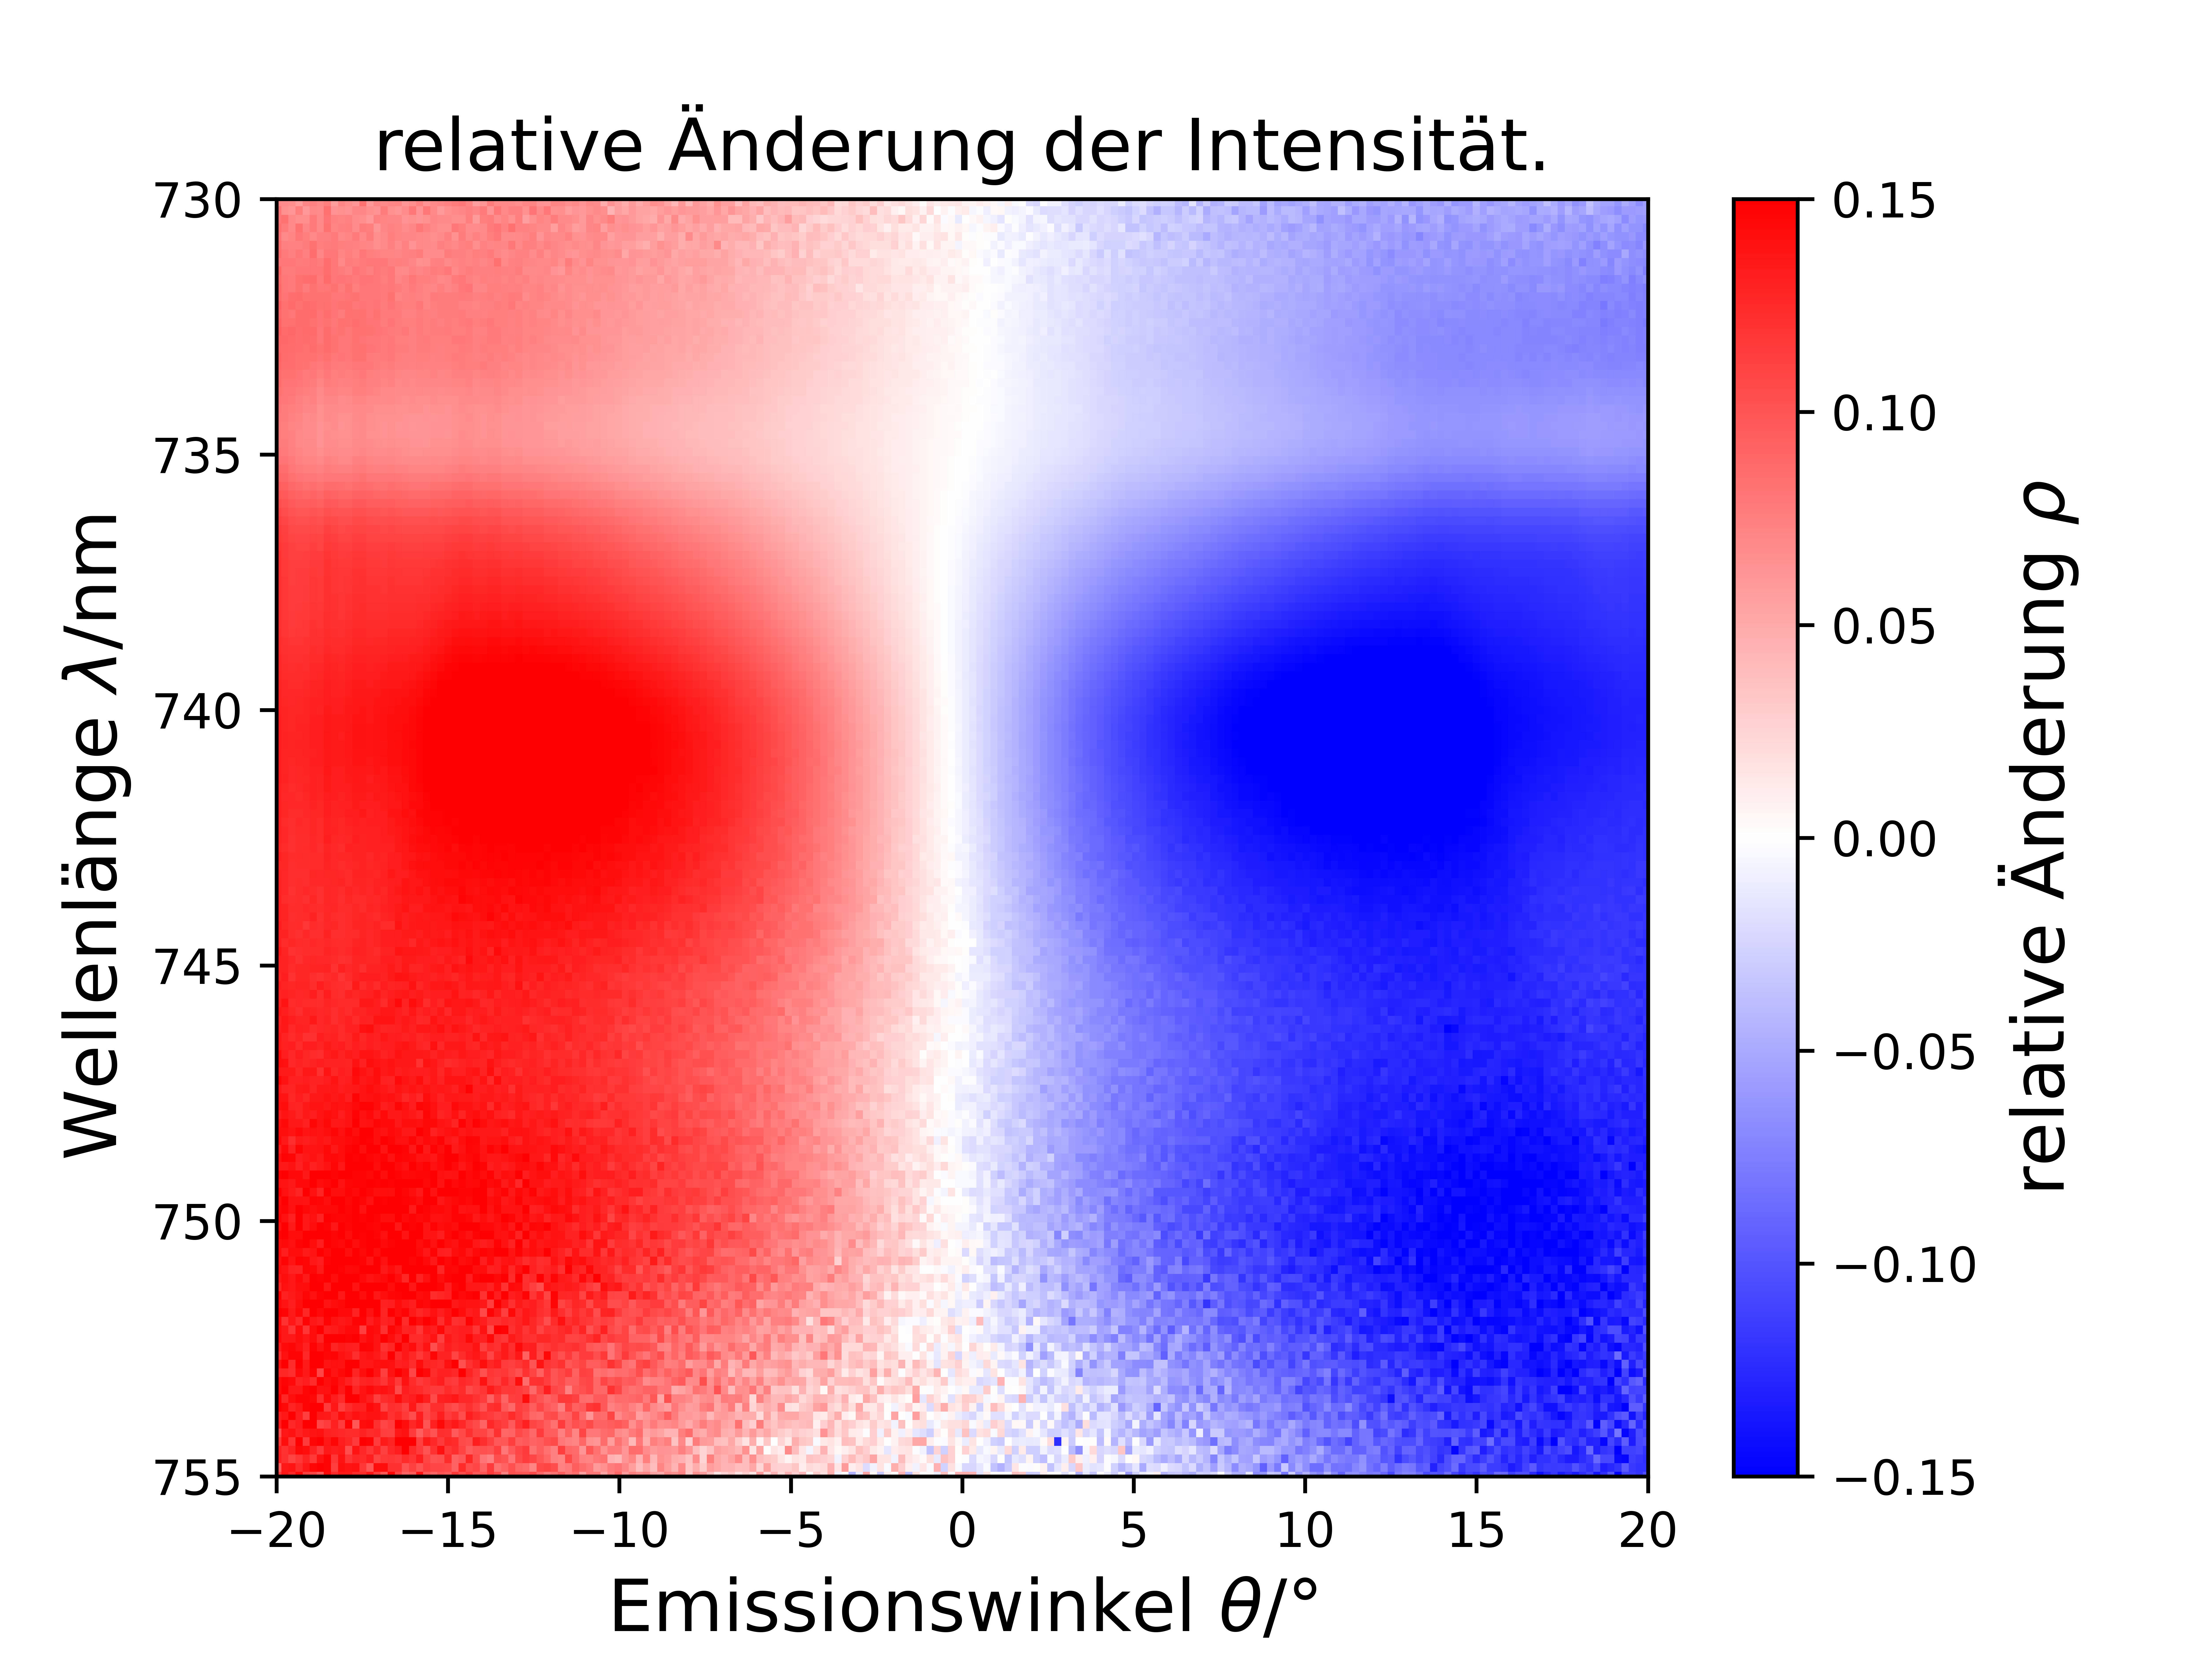
\includegraphics[scale=0.4]{images/colormap_rel_change_intensity_022818A 250nm 4K 2020-07-14.png}\\[-0.5\baselineskip]%           
            }%
        \end{column}
    \end{columns}
\end{frame}


\begin{frame}{Relative Änderung bei \SI{4}{\kelvin}}
    %\pause
    \begin{columns}
        \begin{column}{0.5\textwidth}
            \begin{itemize}
                \item <1-> relative Änderung $\rho$ in Abhängigkeit von Emissionswinkel $\theta$
                \item <2-> antisymmetrisch bis auf eine kleine Abweichung am Nullpunkt 
                \item <3-> Antisymmetrie von Theorie vorhergesagt und bestätigt
                \bigskip
                \item <4-> Definition: Direktionalität
                \begin{equation*}
                    C= \frac{\rho(-\theta)-\rho(\theta)}{2}                    
                \end{equation*}
                \item <6-> steigende Verbesserung der Steuerbarkeit der Lichtemission bis $\theta = \pm \SI{13,5}{\degree}$
            \end{itemize}
        \end{column}
        \begin{column}{0.5\textwidth}
            \centering 
            \only <1-4> {%
            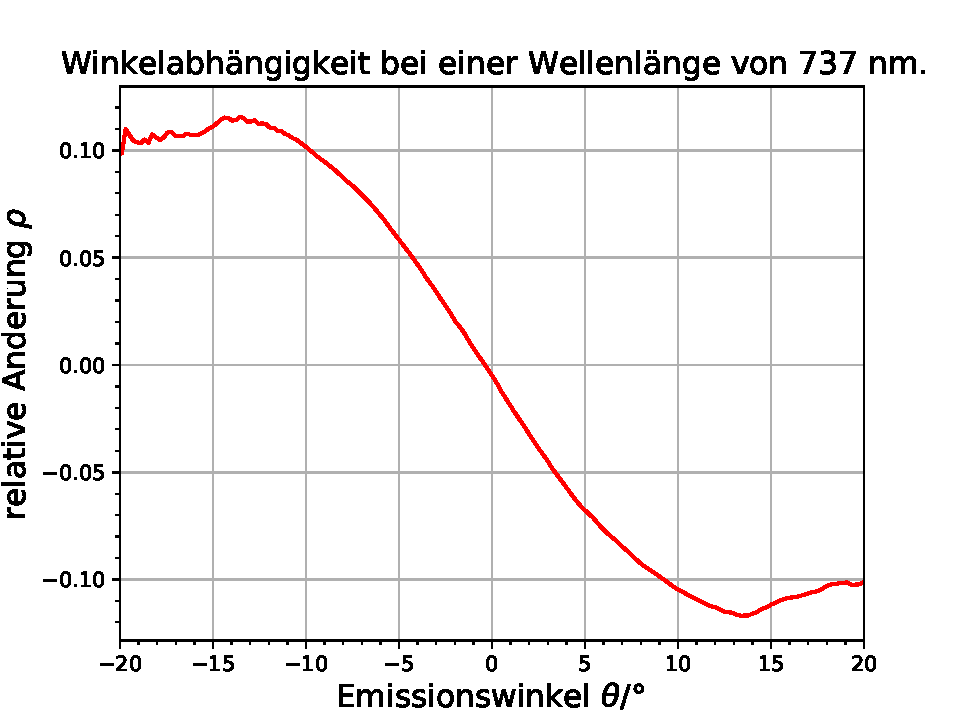
\includegraphics[scale=0.4]{images/rho_at_specific_wavelength_737_nm_022818A 250nm 4K 2020-07-14.pdf}\\[-0.5\baselineskip]%
            }%
            \only <5-> {%
            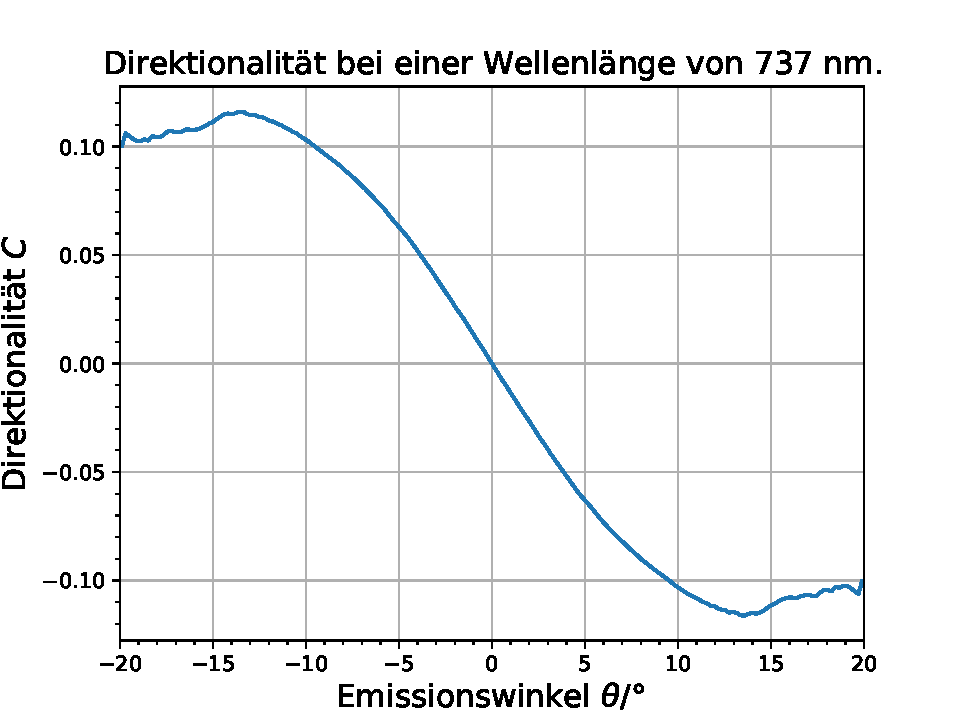
\includegraphics[scale=0.4]{images/rho_at_specific_wavelength_737_nm_022818A 250nm 4K 2020-07-14_korrigiert.pdf}\\[-0.5\baselineskip]%           
            }%
        \end{column}
    \end{columns}
\end{frame}

%\subsection{Temperaturabhängigkeit der Direktionalität}
\begin{frame}{Temperaturabhängigkeit der Direktionalität}
    %\pause^
    \begin{columns}
        \begin{column}{0.5\textwidth}
            \begin{itemize}
                \item <1-> Temperaturbereich $T = \SI{4}{\kelvin}\text{ bis }T = \SI{45}{\kelvin}$
                \bigskip
                \item <2-> Grad der zirkularen Polarisation sinkt mit steigender Temperatur
                \begin{align*}
                    P_c \approx \frac{2}{3} \frac{\Delta_\text{h,F}(T)}{\Delta_\text{lh}} \propto B
                \end{align*}
                \rightarrow Direktionalität sinkt                
                \rightarrow Bestätigung der vorrangestellten Theorie
            \end{itemize}
        \end{column}
        \begin{column}{0.5\textwidth}
            \centering 
            \only <1-> {%
            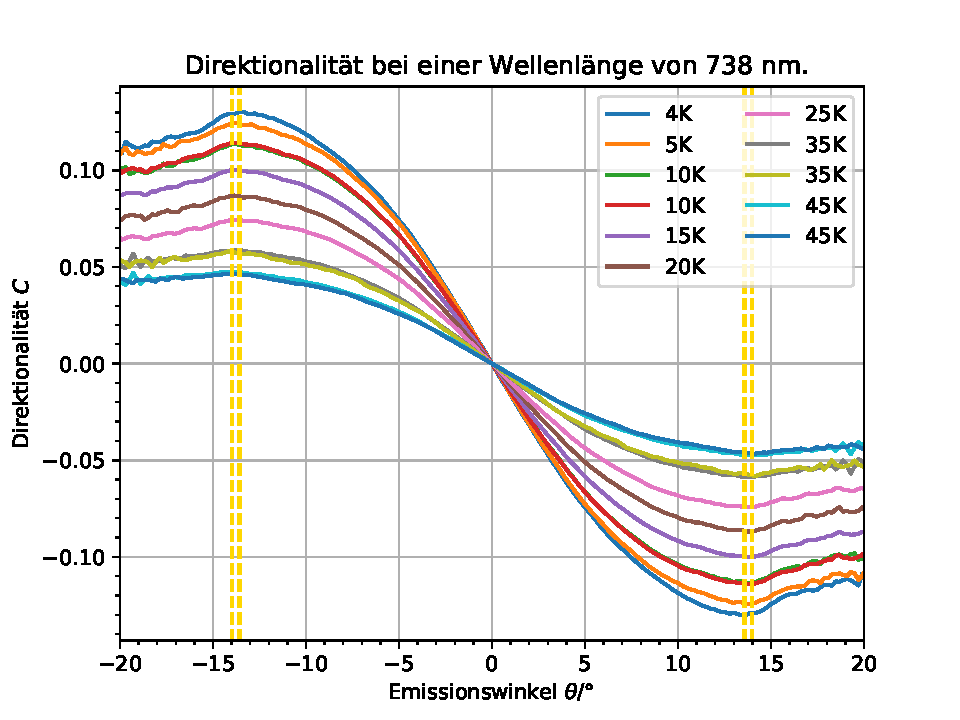
\includegraphics[scale=0.4]{images/Temperaturabhaengigkeit_rho_at_738_nm_4K5K10K10K15K20K25K35K35K45K45K_korrigiert.pdf}\\[-0.5\baselineskip]%
            }%
        \end{column}
    \end{columns}
\end{frame}

\begin{frame}{Temperaturabhängigkeit der Direktionalität}
    %\pause
    \begin{columns}
        \begin{column}{0.5\textwidth}
            \begin{itemize}       
                \item <1-> Fitfunktion
                \begin{align*}
                    C(T)&= C_0 B_\text{$\frac{5}{2}$} \left( \frac{5}{2}\frac{g_\text{Mn} \mu_\text{B} B }{T^*_\text{eff} k_\text{B}}\right)\text{,} \\
                    T^*_\text{eff} &= T + T_0 + T_\text{off}
                \end{align*}
                \item <2->  
                %\begin{align*}
                    $T: \text{gemessene/eingestellte Temperatur}$
                    $T_0:  \text{Offset durch Mangan-Paare }$
                    $T_\text{off}: \text{Offset durch äußere Einflüsse}$
                %\end{align*}
                \item <3-> Fitparameter
                \begin{align*}
                    C_0 & = \si{4,5 \pm 0,3} \\
                    T_\text{off} & = \SI{ 20 \pm 2}{\kelvin}
                \end{align*}
            \end{itemize}
        \end{column}
        \begin{column}{0.5\textwidth}
            \centering 
            \only <1-> {%
            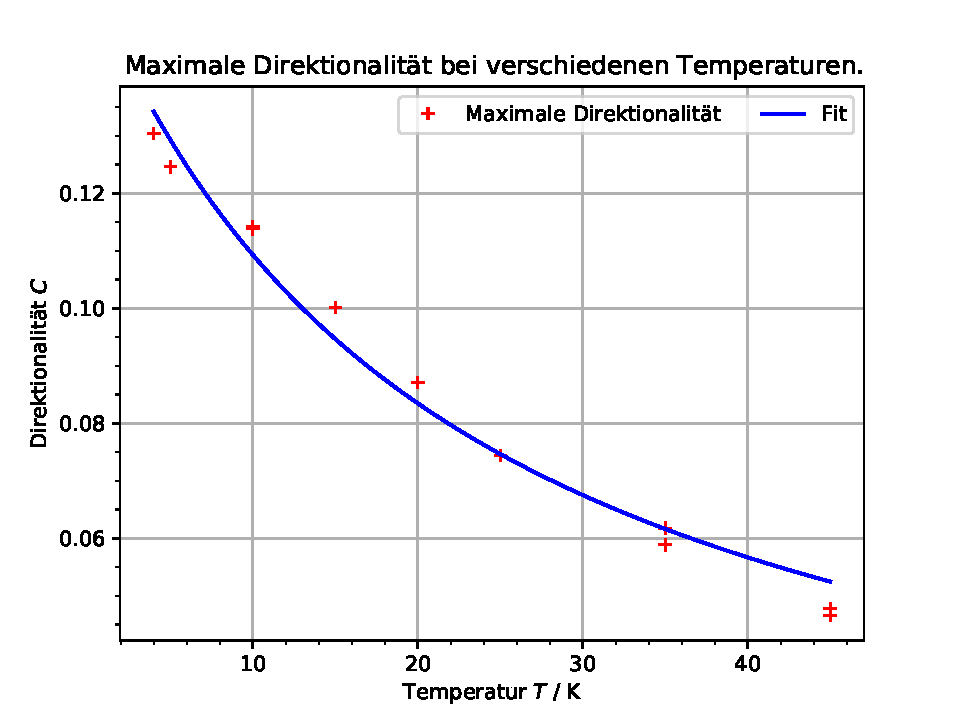
\includegraphics[scale=0.4]{images/Maximale_Rho_bei_Temperaturabhänigkeit.pdf}\\[-0.5\baselineskip]%
            }%
        \end{column}
    \end{columns}
\end{frame}

\begin{frame}{Temperaturabhängigkeit der Direktionalität}
    \begin{columns}
        \begin{column}{0.5\textwidth}
            \begin{itemize} 
                %\item Fitparameter             
                %\begin{align*} 
                %    C_0 & = \si{4,5 \pm 0,3} \\
                %    T_\text{off} & = \SI{ 20 \pm 2}{\kelvin}
                %\end{align*}
                \item <1-> Temperatur Offset $T_\text{off}  = \SI{ 20 \pm 2}{\kelvin}$ relativ groß
                \bigskip
                \item <2-> mögliche Ursache?\\ Leistungsdichte Laser $\SI{400}{\watt\per\centi\meter^2}$
                \rightarrow lokale Temperaturerhöhungen,\\ Temperatursensor nicht auf Probenoberfläche 
                \item <3-> Experiment also schlecht? 
                \bigskip
                \item <4-> Nein! \rightarrow klarer Zusammenhang zwischen Temperatur und Direktionalität
                \bigskip
                \item <5-> Temperaturabhängigkeit kann mit Gleichung gut approximiert werden \rightarrow 
                Verlauf der Direktionalität erkennbar 
            \end{itemize}
        \end{column}
        \begin{column}{0.5\textwidth}
            \centering
            \only <1-> {%
            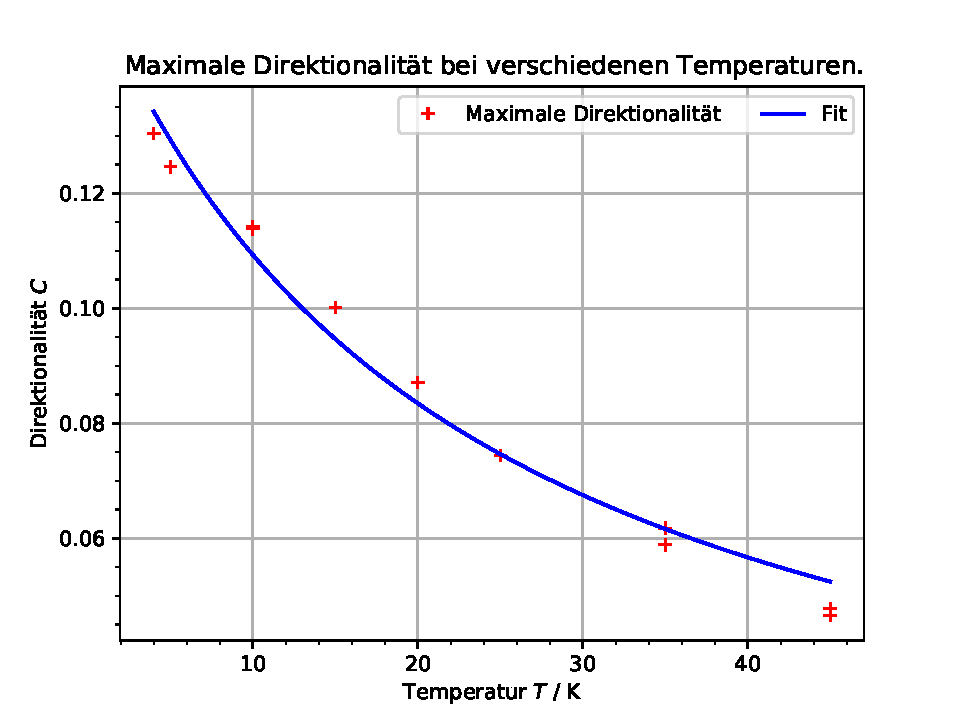
\includegraphics[scale=0.4]{images/Maximale_Rho_bei_Temperaturabhänigkeit.pdf}\\[-0.5\baselineskip]% 
            }%
        \end{column}
    \end{columns}
\end{frame}

\begin{frame}{Verbesserungen und Ausblick}
    \begin{columns}
        \begin{column}{0.5\textwidth}
            \begin{itemize}                 
                \item <1-> Verbesserungen?
                %\bigskip
                \item <2-> Messwerte pendeln um Fit 
                %\bigskip
                \begin{itemize}
                    \item <3-> \rightarrow bessere Approximation möglich
                    \item <4-> weitere Temperaturmessungen 
                \end{itemize}
                \bigskip
                \item <5-> Abhängigkeit der Leistungsdichte des Lasers
                %\bigskip
                \item <6-> Position Temperatursensor
                %\bigskip
                \item <7-> Rolle der Gitterperiode %\vspace{0.3cm}%\\~\\
                %\bigskip
                \item <8-> Zeemanaufspaltung unabhängig der Temperatur, InGaAs/InAlAs? 
            \end{itemize}
        \end{column}
        \begin{column}{0.5\textwidth}
            \centering
            \only <1-> {%
            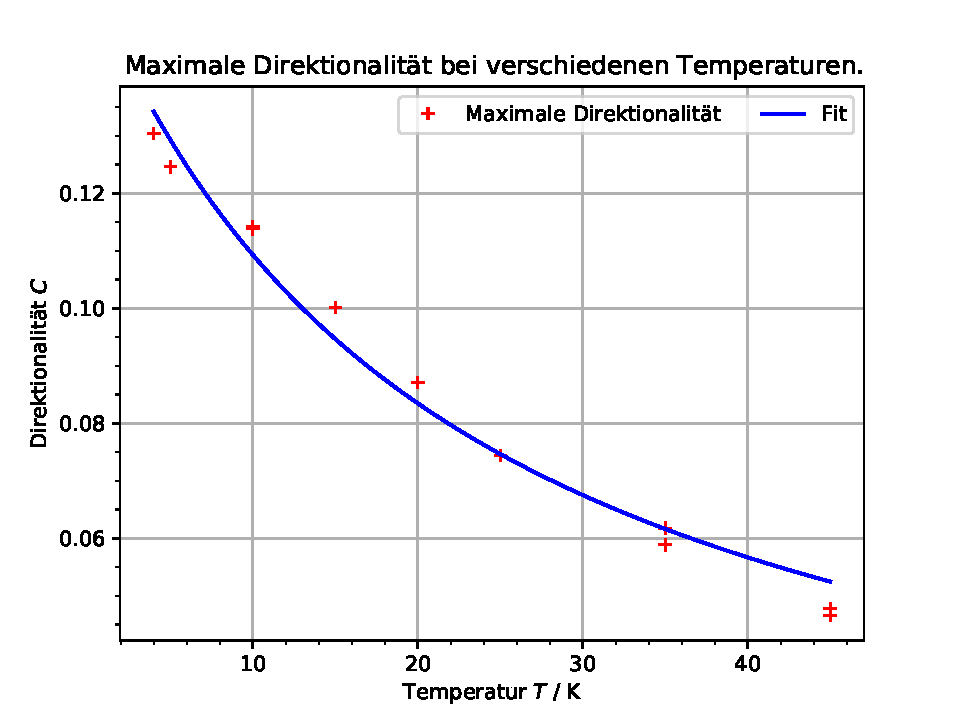
\includegraphics[scale=0.4]{images/Maximale_Rho_bei_Temperaturabhänigkeit.pdf}\\[-0.5\baselineskip]%
            }%
        \end{column}
    \end{columns}
\end{frame}

%\begin{frame}{Zusammenfassung}
%    \begin{itemize}
%        \item ja
%    \end{itemize}       
%\end{frame}

%\section{Ende}
\begin{frame}
    Danke für Ihre Aufmerksamkeit
\end{frame}


\begin{frame}{Backup}
    \centering
    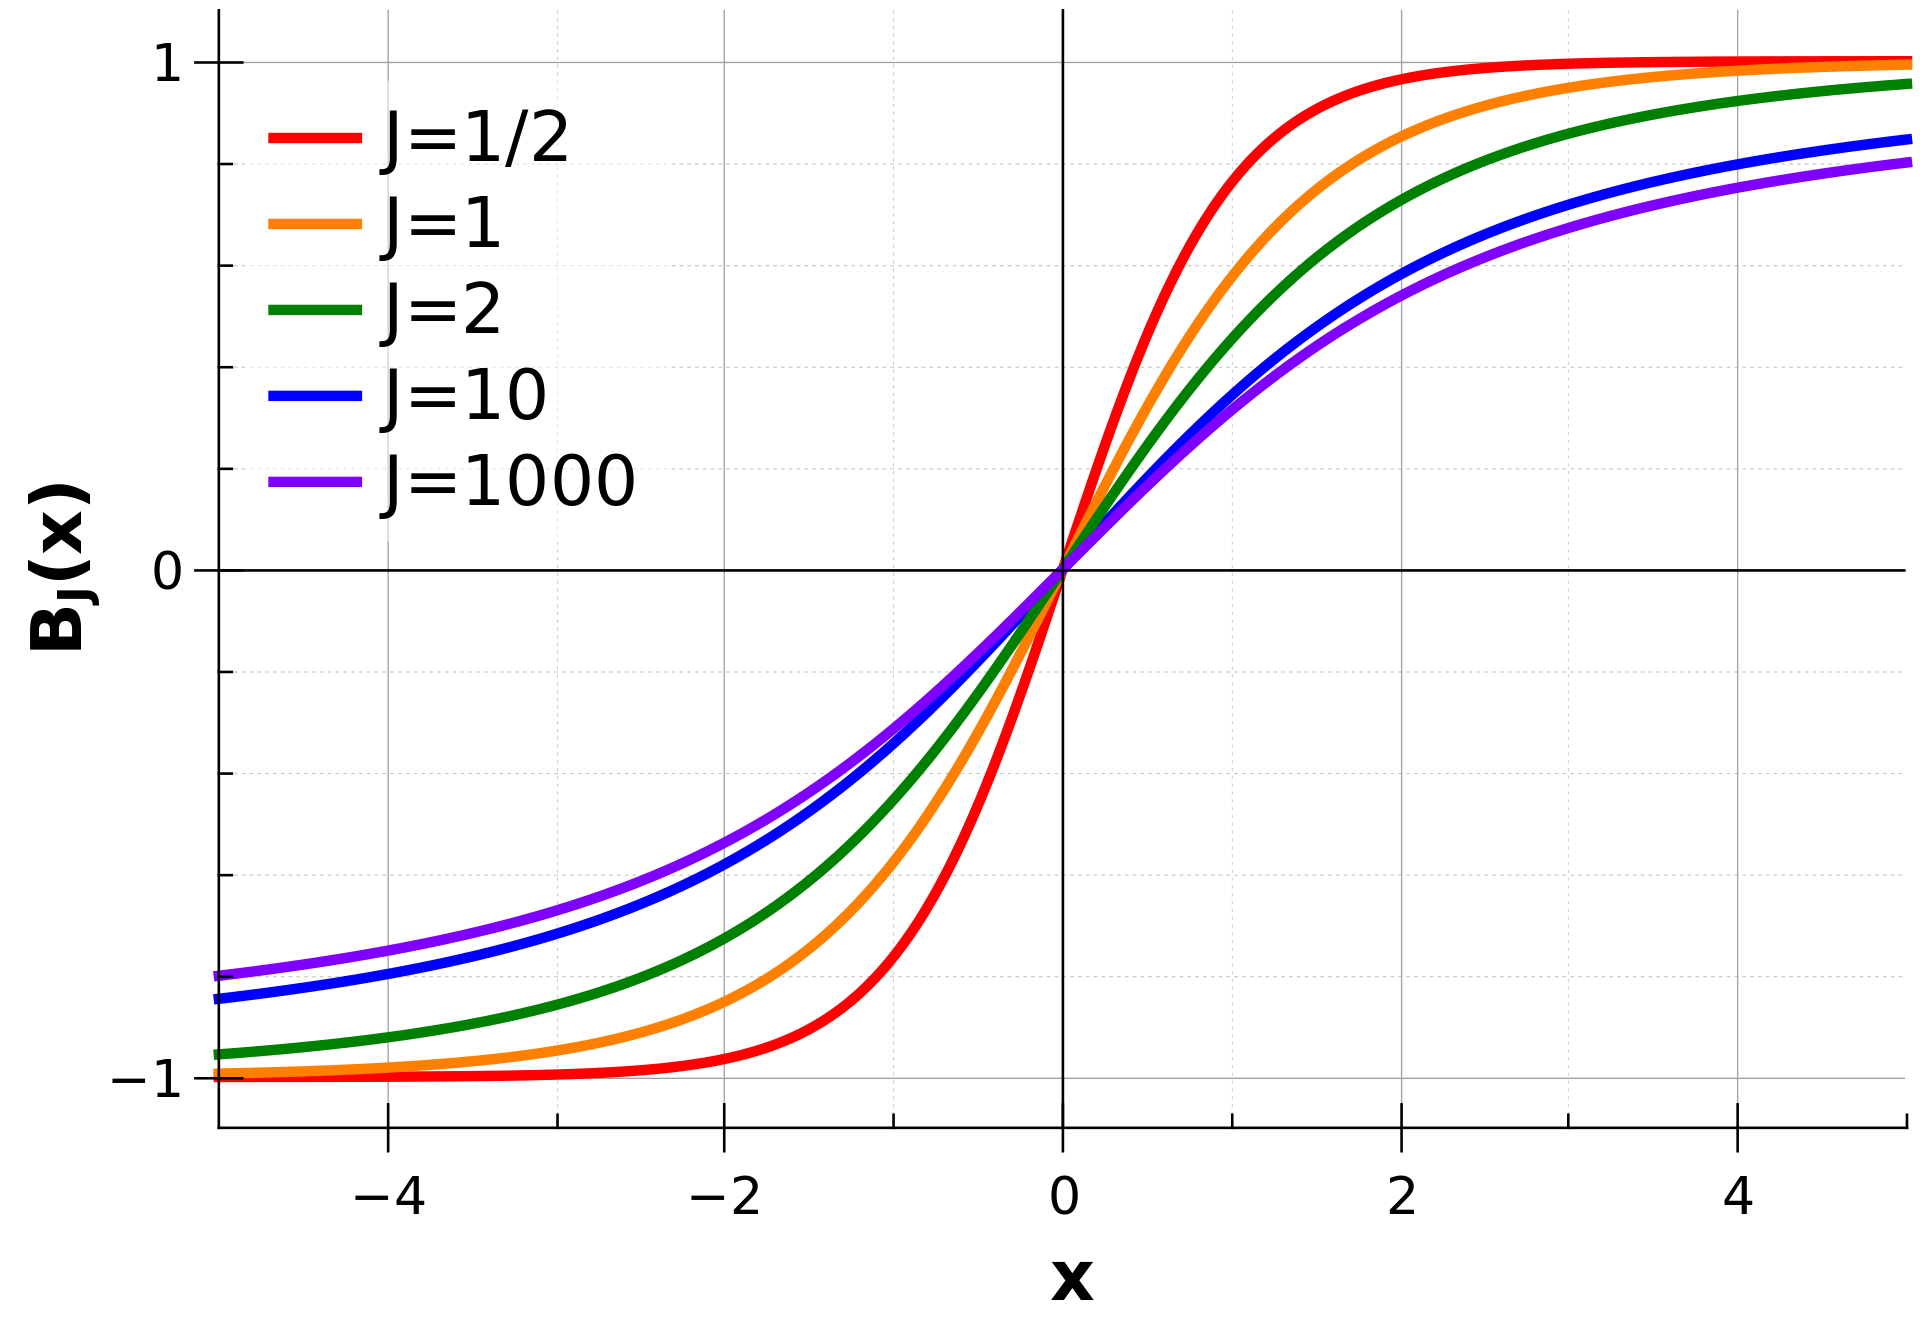
\includegraphics[scale=0.15]{images/b.png}\\[-0.5\baselineskip]
\end{frame}

\begin{frame}{Backup}
    \centering
    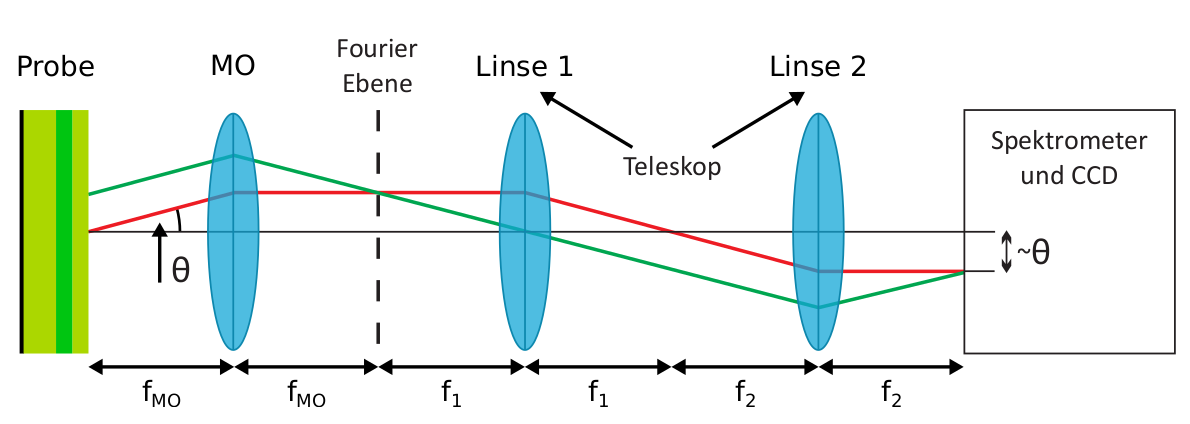
\includegraphics[scale=0.3]{images/lars.png}\\[-0.5\baselineskip]
\end{frame}